\documentclass[11pt]{article}

\renewcommand\familydefault{\sfdefault}
 
%input preamble and macros
% \input{../slides/macros/preamble}
\usepackage{etex} % fixes new-dimension error
\usepackage{lmodern}
\usepackage[T1]{fontenc}

%----------------------------------------------------------------------------
\usepackage{graphicx,amsmath}
\usepackage{stmaryrd} % cf. interleave
\usepackage{booktabs}
\usepackage{amscd}
\usepackage{multicol}
\usepackage[absolute,overlay]{textpos}
\usepackage{alltt}
\usepackage{proof}
\usepackage{subcaption}
\usepackage{tikz}
\usepackage{tikz-cd}
\usepackage[new]{old-arrows}
\usepackage[all]{xy}
\usepackage{pgfplots}
\usepackage{textcomp}


\usepackage{transparent}
\usepackage{xspace}
\usepackage{listings}
\usepackage{pdfpages}
\usepackage{relsize}

%%%%%%%%%%%%% Macros
\newcommand{\Ban}{\catfont{Ban}}
\newcommand{\Met}{\catfont{Met}}
\newcommand{\Shuff}{\mathrm{Sf}}
\newcommand{\Cats}{\catfont{Cat}}
\newcommand{\VCat}{\mathcal{V}\text{-}\Cats}
\newcommand{\VCatSy}{\mathcal{V}\text{-}\Cats_{\mathsf{sym}}}
\newcommand{\VCatSe}{\mathcal{V}\text{-}\Cats_{\mathsf{sep}}}
\newcommand{\VCatSS}{\mathcal{V}\text{-}\Cats_{\mathsf{sym,sep}}}
%%%% Categories
\newcommand{\catfont}[1]{\mathsf{#1}}
\newcommand{\cop}{\catfont{op}}
\newcommand{\Law}{\catfont{Law}}
\newcommand{\catV}{\catfont{V}}
\newcommand{\catX}{\catfont{X}}
\newcommand{\catC}{\catfont{C}}
\newcommand{\catD}{\catfont{D}}
\newcommand{\catA}{\catfont{A}}
\newcommand{\catB}{\catfont{B}}
\newcommand{\catI}{\catfont{I}}
\newcommand{\Set}{\catfont{Set}}
\newcommand{\Top}{\catfont{Top}}
\newcommand{\Pos}{\catfont{Pos}}
\newcommand{\Inj}{\catfont{Inj}}
\newcommand{\Det}{\catfont{RMhat}}
\newcommand{\CoAlg}[1]{\catfont{CoAlg}\left (#1 \right )}
\newcommand{\Mon}{\catfont{Mon}}
\newcommand{\Mnd}{\catfont{Mnd}(\catC)}
\newcommand{\SMnd}{\catfont{Mnd}(\Set)}
\newcommand{\CLat}{\catfont{CLat}}
\newcommand{\Stone}{\catfont{Stone}}
\newcommand{\Spectral}{\catfont{Spectral}}
\newcommand{\CompHaus}{\catfont{CompHaus}}
\newcommand{\Subs}[2]{\catfont{Sub}_{}}
\newcommand{\Cone}{\catfont{Cone}}
\newcommand{\StComp}{\catfont{StablyComp}}
\newcommand{\PosC}{\catfont{PosComp}}
\newcommand{\Haus}{\catfont{Haus}}
\newcommand{\Meas}{\catfont{Meas}}
\newcommand{\Ord}{\catfont{Ord}}
\newcommand{\EndoC}{[\catC,\catC]}
%% General functors
\newcommand{\funfont}[1]{#1}
\newcommand{\funF}{\funfont{F}}
\newcommand{\funU}{\funfont{U}}
\newcommand{\funG}{\funfont{G}}
\newcommand{\funT}{\funfont{T}}
\newcommand{\funI}{\funfont{I}}
%% Particular kinds of functors
\newcommand{\sfunfont}[1]{\mathrm{#1}}
\newcommand{\Pow}{\sfunfont{P}}
\newcommand{\Dist}{\sfunfont{D}}
\newcommand{\Maybe}{\sfunfont{M}}
\newcommand{\List}{\sfunfont{L}}
\newcommand{\UForg}{\sfunfont{U}}
\newcommand{\Forg}[1]{\sfunfont{U}_{#1}}
\newcommand{\Id}{\sfunfont{Id}}
\newcommand{\Vie}{\sfunfont{V}}
\newcommand{\Disc}{\funfont{D}}
\newcommand{\Weight}{\sfunfont{W}}
\newcommand{\homf}{\sfunfont{hom}}
\newcommand{\Yoneda}{\sfunfont{Y}}
%% Diagram functors
\newcommand{\Diag}{\mathscr{D}}
\newcommand{\KDiag}{\mathscr{K}}
\newcommand{\LDiag}{\mathscr{L}}
%% Monads
\newcommand{\monadfont}[1]{\mathbb{#1}}
\newcommand{\monadT}{\monadfont{T}}
\newcommand{\monadS}{\monadfont{S}}
\newcommand{\monadU}{\monadfont{U}}
\newcommand{\monadH}{\monadfont{H}}
\newcommand{\str}{\mathrm{str}}
%% Adjunctions
\newcommand\adjunct[2]{\xymatrix@=8ex{\ar@{}[r]|{\top}\ar@<1mm>@/^2mm/[r]^{{#2}}
& \ar@<1mm>@/^2mm/[l]^{{#1}}}}
\newcommand\adjunctop[2]{\xymatrix@=8ex{\ar@{}[r]|{\bot}\ar@<1mm>@/^2mm/[r]^{{#2}}
& \ar@<1mm>@/^2mm/[l]^{{#1}}}}
%% Retractions
\newcommand\retract[2]{\xymatrix@=8ex{\ar@{}[r]|{}\ar@<1mm>@/^2mm/@{^{(}->}[r]^{{#2}}
& \ar@<1mm>@/^2mm/@{->>}[l]^{{#1}}}}
%% Limits
\newcommand{\pv}[2]{\langle #1, #2 \rangle}
\newcommand{\limt}{\mathrm{lim}}
\newcommand{\pullbackcorner}[1][dr]{\save*!/#1+1.2pc/#1:(1,-1)@^{|-}\restore}
\newcommand{\pushoutcorner}[1][dr]{\save*!/#1-1.2pc/#1:(-1,1)@^{|-}\restore}
%% Colimits
\newcommand{\colim}{\mathrm{colim}}
\newcommand{\inl}{\mathrm{inl}}
\newcommand{\inr}{\mathrm{inr}}
%% Distributive categories
\newcommand{\distr}{\mathrm{dist}}
\newcommand{\undistr}{\mathrm{undist}}
%% Closedness
\newcommand{\curry}[1]{\mathrm{curry}{#1}}
\newcommand{\app}{\mathrm{app}}
%% Misc. operations
\newcommand{\const}[1]{\underline{#1}}
\newcommand{\comp}{\cdot}
\newcommand{\id}{\mathrm{id}}
%% Factorisations
\newcommand{\EClass}{E}
\newcommand{\MClass}{M}
\newcommand{\MConeClass}{\mathcal{M}}
%%%%%%%%%%%%%%%% End of Categorical Stuff

%%%% Misc
%% Operations
\newcommand{\blank}{\, - \,}
\newcommand{\sem}[1]{\llbracket #1 \rrbracket}
\newcommand{\closure}[1]{\overline{#1}}
% \DeclareMathOperator{\img}{\mathrm{im}}
% \DeclareMathOperator{\dom}{\mathrm{dom}}
% \DeclareMathOperator{\codom}{\mathrm{codom}}
%% Sets of numbers
\newcommand{\N}{\mathbb{N}}
\newcommand{\Z}{\mathbb{Z}}
\newcommand{\Nats}{\mathbb{N}}
\newcommand{\Reals}{\mathbb{R}}
\newcommand{\Rz}{\Reals_{\geq 0}}
\newcommand{\Complex}{\mathbb{C}}
%% Writing
\newcommand{\cf}{\emph{cf.}}
\newcommand{\ie}{\emph{i.e.}}
\newcommand{\eg}{\emph{e.g.}}
\newcommand{\df}[1]{\emph{\textbf{#1}}}
%%%%%%%%%%%%%%%% End of Misc

%%%% Programming Stuff
%% Types
\newcommand{\typefont}[1]{\mathbb{#1}}
\newcommand{\typeOne}{1}
\newcommand{\typeTwo}{2}
\newcommand{\typeA}{\typefont{A}}
\newcommand{\typeX}{\typefont{X}}
\newcommand{\typeB}{\typefont{B}}
\newcommand{\typeC}{\typefont{C}}
\newcommand{\typeV}{\typefont{V}}
\newcommand{\typeD}{\typefont{D}}
\newcommand{\typeI}{\typefont{I}}
%% RuleName
\newcommand{\rulename}[1]{(\mathrm{#1})}
%% Sequents
\newcommand{\jud}{\vdash}
\newcommand{\vljud}{\rhd}
\newcommand{\cojud}{\vdash_{\co}}
\newcommand{\vl}{\mathtt{v}}
\newcommand{\co}{\mathtt{c}}
% Program font
\newcommand{\prog}[1]{\mathtt{#1}}
\newcommand{\pseq}[3]{#1 \leftarrow #2; #3}
\newcommand{\ppm}[4]{(#1,#2) \leftarrow #3; #4}
\newcommand{\pinl}[1]{\prog{inl}(#1)}
\newcommand{\pinr}[1]{\prog{inr}(#1)}
\newcommand{\pcase}[4]{\prog{ case } #1 \prog{ of } \pinl{#2} \Rightarrow #3 ; \pinr{#2} \Rightarrow #4}
%% Sets of terms
\newcommand{\ValuesBP}[2]{\mathsf{Values}(#1, #2)}
\newcommand{\TermsBP}[2]{\mathsf{Terms}(#1, #2)}
\newcommand{\closValP}[1]{\ValuesBP{\emptyset}{#1}}
\newcommand{\closTermP}[1]{\TermsBP{\emptyset}{#1}}
\newcommand{\closVal}{\closValP{\typeA}}
\newcommand{\closTerm}{\closTermP{\typeA}}
%% Contextual equivalence
\newcommand{\ctxeq}{\equiv_{\prog{ctx}}}
%%%% End of Programming Stuff

%------ Setting lecture info ----------------------------------------------
\newcounter{lectureID}
\stepcounter{lectureID}
\newcommand{\getLecture}{\arabic{lectureID}\xspace}
\newcommand{\setLectureBasic}[1]{
  \title{
    #1
    }
  \author{Jos\'{e} Proen\c{c}a}
  \institute{CISTER -- U.Porto, Porto, Portugal
            \hfill 
            \begin{tabular}{r@{}}
            \url{https://fm-dcc.github.io/sv2425}
            \end{tabular}
            }
  \date{System Verification (CC4084) 2024/2025}
  % logos of institutions
  \titlegraphic{
    \begin{textblock*}{5cm}(4.0cm,6.80cm)
       
\includegraphics[scale=0.18]{images/fcup}\hspace*{.85cm}~%
    \end{textblock*}
    \begin{textblock*}{5cm}(8.4cm,7.25cm)
      % \includegraphics[scale=0.50]{images/dcc}
      
\includegraphics[scale=0.20]{images/cister}
    \end{textblock*}
  }  
}
\newcommand{\setLecture}[2]{\setcounter{lectureID}{#1}\setLectureBasic{#1. #2}}

%------ Counters for exercises ----------------------------------------------
\newcounter{cExercise}
\newcommand{\exercise}{\stepcounter{cExercise}Ex.\,\arabic{lectureID}.\arabic{cExercise}:\xspace}
\newcommand{\exerciseBack}{\addtocounter{cExercise}{-1}}
\newcommand{\exerciseAdd}{\stepcounter{cExercise}}
\newcommand{\doExercise}[3][0mm]{\begin{exampleblock}{\exercise #2}\wrap{\rule{0pt}{#1}}#3\end{exampleblock}}
\newcommand{\doSimpleExercise}[2][0mm]{\begin{exampleblock}{}\wrap{\rule{0pt}{#1}}\structure{\textbf{\exercise} #2}\end{exampleblock}}

% Slide
\newenvironment{slide}[1]{\begin{frame}\frametitle{#1}}{\end{frame}}

% Misc by José
\newcommand{\wrap}[2][]{\begin{tabular}[#1]{@{}c@{}}#2\end{tabular}}
\newcommand{\mwrap}[1]{\ensuremath{\begin{array}{@{}c@{}}#1\end{array}}}
\def\trans#1{\xrightarrow{#1}}  % - a - > 
\def\Trans#1{\stackrel{#1}{\Longrightarrow}} % =a=> 
\newcommand{\transp}[2][35]{\color{fg!#1}#2}
\newcommand{\transpt}[2][.35]{\tikz{\node[inner sep=1pt,fill opacity=0.5]{#2}}}
\newcommand{\faded}[2][0.4]{{\transparent{#1}#2}} % alternative to "transp" using transparent package
\newcommand{\set}[1]{\left\{ #1 \right\}} % {a,b,...z}
\newcommand{\mi}[1]{\ensuremath{\mathit{#1}}\xspace}
\newcommand{\mf}[1]{\ensuremath{\mathsf{#1}}\xspace}
% \newcommand{\gold}[1]{\textcolor{darkgoldenrod}{#1}\xspace}


%------ using color ---------------------------------------------------------
\definecolor{goldenrod}{rgb}{.80392 .60784 .11373}
\definecolor{darkgoldenrod}{rgb}{.5451 .39608 .03137}
\definecolor{brown}{rgb}{.15 .15 .15}
\definecolor{darkolivegreen}{rgb}{.33333 .41961 .18431}
\definecolor{myGray}{gray}{0.85}
%
%
\newcommand{\red}[1]{\textcolor{red!80!black}{#1}\xspace}
\newcommand{\blue}[1]{\textcolor{blue}{#1}\xspace}
\newcommand{\gold}[1]{\textcolor{darkgoldenrod}{#1}\xspace}
\newcommand{\gray}[1]{\textcolor{myGray}{#1}\xspace}
% \def\alert#1{{\darkgoldenrod #1}}
% \def\alert#1{{\alert{#1}}}
%\def\brw#1{{\brown #1}}
% \def\structure#1{{\blue #1}}
% \def\tstructure#1{\textbf{\darkblue #1}}
%%\def\gre#1{{\green #1}}
\def\gre#1{{\darkolivegreen #1}}
\def\gry#1{{\textcolor{gray}{#1}}}
\def\rdb#1{{\red #1}}
\def\st{\mathbf{.}\,}
\def\laplace#1#2{*\txt{\mbox{ \fcolorbox{black}{myGray}{$\begin{array}{c}\mbox{#1}\\\\#2\\\\\end{array}$} }}}
%\newcommand{\galois}[2]{#1\; \dashv\; #2}



% ----- from LSB
\def\Act{N}
\def\cnil{\mathbf{0}}
\def\cpf#1#2{#1 . #2}                           % a.P
\def\cou#1#2{#1 \mathbin{+} #2}                 % P + Q
%\def\crt#1#2{\mathbin{#1 \setminus_{#2}}}       % P \ A
%\def\crtt#1#2{\mathbin{#1 \setminus\!\setminus_{#2}}}       % P \ A
%\def\crt#1#2{\mathsf{new}\, #2\;  #1}       % P \ A
\def\crt#1#2{#1 \backslash #2}       % P \ A
%\def\crn#1#2{\{#2\}\, #1}                  % P[f]
\def\ainv#1{\overline{#1}}
\def\rtran#1{\stackrel{#1}{\longrightarrow}}
% \def\pair#1{\const{#1}}
\def\pair#1{\langle #1 \rangle}
\def\asor{\mathbin{|}}                    % A | B
\def\setdef#1#2{\mathopen{\{} #1 \asor #2 \mathclose{\}}}
\def\imp{\mathbin{\Rightarrow}}
\def\dimp{\mathbin{\Leftrightarrow}}
\def\rimp{\mathbin{\Leftarrow}}
\def\rra{\longrightarrow}
\def\rcb#1#2#3#4{\def\nothing{}\def\range{#3}\mathopen{\langle}#1 \ #2 \ \ifx\range\nothing::\else: \ #3 :\fi \ #4\mathclose{\rangle}}
\def\aconv#1{#1^{\circ}} 
\def\abv{\stackrel{\rm abv}{=}}


\def\crn#1#2{\mathbin{#1[#2]}}                  % P[f]
\def\couit#1#2{\Sigma_{#1}#2}                  %  + i=1,n
\def\cpar#1#2{#1 \mid #2}                       %  |
\def\ctpar#1#2{#1 \parallel #2}                       %  |
\def\cpars#1#2#3{#1 \mid_{#3} #2}               %  |S

% Spliting frames in 2 columns
\newcommand{\splittwo}[4]{ 
  \begin{columns}[T]% align columns
  \begin{column}{#1\textwidth} #3 \end{column} ~~~
  \begin{column}{#2\textwidth} #4 \end{column} \end{columns}
}
\newcommand{\frsplit}[3][.48]{
  \begin{columns}%[T] % align columns
  \begin{column}{#1\textwidth} #2 \end{column} ~~~
  \begin{column}{#1\textwidth} #3 \end{column} \end{columns}
}
\newcommand{\frsplitdiff}[5][]{
  \begin{columns}[#1]%[T] % align columns
  \begin{column}{#2\textwidth} #4 \end{column} ~~~
  \begin{column}{#3\textwidth} #5 \end{column} \end{columns}
}
\newcommand{\frsplitt}[3][.48]{
  \begin{columns}[T] % align columns
  \begin{column}{#1\textwidth} #2 \end{column} ~~~
  \begin{column}{#1\textwidth} #3 \end{column} \end{columns}
}
\newcommand{\col}[2][.48]{\begin{column}{#1\textwidth} #2 \end{column}}
\newcommand{\colb}[3][.48]{\begin{column}{#1\textwidth} \begin{block}{#2} #3 \end{block} \end{column}}

% Spliting frames in 3 columns
\newcommand{\splitthree}[6]{
  \begin{columns}[T] % align columns
  \begin{column}{#1\textwidth} #4 \end{column} ~~~
  \begin{column}{#2\textwidth} #5 \end{column} ~~~
  \begin{column}{#3\textwidth} #6 \end{column} \end{columns}
}
\newcommand{\frsplitthree}[4][.31]{
  \begin{columns}%[T] % align columns
  \begin{column}{#1\textwidth} #2 \end{column} ~~~
  \begin{column}{#1\textwidth} #3 \end{column} ~~~
  \begin{column}{#1\textwidth} #4 \end{column} \end{columns}
}
\newcommand{\frsplitdiffthree}[5]{
  \begin{columns}%[T] % align columns
  \begin{column}{#1\textwidth} #3 \end{column} ~~~
  \begin{column}{#1\textwidth} #4 \end{column} ~~~
  \begin{column}{#2\textwidth} #5 \end{column} \end{columns}
}
\newcommand{\frsplittthree}[4][.32]{
  \begin{columns}[T] % align columns
  \begin{column}{#1\textwidth} #2 \end{column} ~
  \begin{column}{#1\textwidth} #3 \end{column} ~
  \begin{column}{#1\textwidth} #4 \end{column} \end{columns}
}


\newcommand{\typerule}[4][]{\ensuremath{\begin{array}[#1]{c}\textsf{\scriptsize ({#2})} \\#3 \\\hline\raisebox{-3pt}{\ensuremath{#4}}\end{array}}}
\newcommand{\styperule}[3][]{\ensuremath{\begin{array}[#1]{c} #2 \\[0.5mm]\hline\raisebox{-4pt}{\ensuremath{#3}}\end{array}}}
\newcommand{\shrk}{\vspace{-3mm}}

\def\caixa#1{\medskip
  \begin{center}
  \fbox{\begin{minipage}{0.9\textwidth}\protect{#1}\end{minipage}}
  \end{center}}

% \newcommand{\mybox}[2][0.9]{
%   \begin{minipage}{#1\textwidth}\begin{block}{}\centering #2\end{block}\end{minipage}}
% \newcommand{\mycbox}[2][0.9]{
%   {\\[-5mm]\centering\mybox[#1]{#2}\\[-5mm]}}
\newcommand{\mybox}[2][4mm]{
  % \begin{minipage}{#1\textwidth}\begin{block}{}\centering #2\end{block}\end{minipage}}
  \tikz{\node[fill=barcolor!40,align=center,inner sep=#1]{#2};}}
\newcommand{\mycbox}[2][4mm]{
  \begin{center}\mybox[#1]{#2}\end{center}}
  % {\\[-5mm]\centering\mybox[#1]{#2}\\[-5mm]}}



%%%%% Tikz
% \usetikzlibrary{arrows.meta, calc, fit, tikzmark}
\usetikzlibrary{%
  positioning
 ,patterns
 ,arrows
 ,arrows.meta
 ,automata
 ,calc
 ,shapes
 ,fit
 ,tikzmark
 ,fadings
 ,decorations.pathreplacing
 ,plotmarks
% ,pgfplots.groupplots
 ,decorations.markings
 ,shadows
}
% \tikzset{shorten >=1pt,node distance=2cm,on grid,auto,initial text={},inner sep=2pt}
\tikzstyle{aut}=[shorten >=1pt,node distance=2cm,on grid,auto,initial text={},inner sep=2pt]
\tikzstyle{st}=[circle,draw=black,fill=black!10,inner sep=3pt]
\tikzstyle{sst}=[rectangle,draw=none,fill=none,inner sep=3pt]
\tikzstyle{final}=[accepting]
\tikzstyle{lbl}=[font=\footnotesize,inner sep=3pt]

% For modal logic and timed automata slides
\def\uppaal{\textsc{Uppaal}}
\def\cc#1{\mathcal{C}(#1)}
% % \newcommand{\pv}[2]{\langle #1 \rangle\, #2}
% \newcommand{\nc}[2]{[#1]\, #2}
\newcommand{\impp}{\mathbin{\rightarrow}}
\newcommand{\dimpp}{\mathbin{\leftrightarrow}}
\newcommand{\always}{\boxempty}
\newcommand{\nexts}{\bigcirc}
\newcommand{\until}{\mathbin{\mathcal U}}
\newcommand{\eventual}{\Diamond}
\newcommand{\true}{\mathsf{true}}
\newcommand{\false}{\mathsf{false}}
\newcommand{\fdec}[3]{#1: #2 \longrightarrow  #3}
\newcommand{\pow}[1]{{\cal P}#1}
\newcommand{\tran}[1]{\stackrel{#1}{\longrightarrow}}
\newcommand{\PP}{\alert{P}}
\newcommand{\universal}[2]{\forall_{#1}\; .\; #2}
\newcommand{\existential}[2]{\exists_{#1}\; .\; #2}
\newcommand{\enset}[1]{\mathopen{ \{ }#1\mathclose{ \} }} % {a,b,...z}
\newcommand{\diam}[1]{\ensuremath{\langle #1 \rangle}}
\newcommand{\boxx}[1]{\ensuremath{[#1]}}
\newcommand{\evm}[1]{\langle #1 \rangle\,}
\newcommand{\alm}[1]{[#1]\,}
\newcommand{\evmb}[1]{\evm{\alert{#1}}}
\newcommand{\almb}[1]{\alm{\alert{#1}}}
\def\R{\mathcal{R}}
\def\TL#1{\mathcal{T}(#1)}

%%% Uppaal-like diagrams
\newcommand{\uppbox}[3][20mm]{\tikz{
  \node[black!15,fill=black!15,minimum width=#1,align=left](title){\textbf{{\footnotesize #2}}};
  \node[black!15,fill=black!15,left,xshift=4mm]at(title.east){\textbf{{\footnotesize #2}}};
  \node[blue!60!cyan,right] at(title.west){\textbf{{\footnotesize #2}}};
  \node[below,inner sep=2mm,fill=white,xshift=2mm](box)at(title.south){\includegraphics[width=#1]{#3}};
  \node[fit=(title)(box),draw=black,inner sep=0pt]{};
}}

\newcommand{\uppboxv}[3][20mm]{\tikz{
  \node[below,inner sep=2mm,fill=white](box){\includegraphics[height=#1]{#3}};
  \coordinate[yshift=5mm](top)at(box.north);
  \node[fit=(top)(box.north west)(box.north east),inner sep=0pt,fill=black!15](title){};
  \node[blue!60!cyan,right] at(title.west){\textbf{{\footnotesize #2}}};
  \node[fit=(title)(box),draw=black,inner sep=0pt]{};
}}
%%% frame for pictures [graphics-options]{content}
\newcommand{\includegraphicsframed}[2][]{\tikz{
  \node[below,inner sep=1mm,fill=barcolor,%xshift=2mm,
    draw=black,
    drop shadow={
      top color=gray,
      bottom color=white,
      %fill=gray,
      opacity=0.2,
      shadow xshift=4pt,
      shadow yshift=-3pt
    }](box){\includegraphics[#1]{#2}};
}}

%% COnfiguring Listings
\lstset{ % basic style
  % language=scala,
  basicstyle=\ttfamily\scriptsize,
  breakatwhitespace=true,
  breaklines=true,
  mathescape,
  % morecomment=[l]{//},
  % morecomment=[n]{/*}{*/},
  % frame=single,                    % adds a frame around the code
  rulecolor=\color{black!40},         % if not set, the frame-color may be changed on line-breaks within not-black text (e.g. comments (green here))
  xleftmargin=1.5mm,
  xrightmargin=1.5mm,
  backgroundcolor=\color{black!5},
  % line numbers
%  numbers=left,  % where to put the line-numbers; possible values are (none, left, right)
 numbersep=5pt, % how far the line-numbers are from the code
 numberstyle=\tiny\color{gray},   
 stepnumber=1,  % the step between two line-numbers. If it is 1 each line will be numbered      
%  xleftmargin=3mm,
%  xrightmargin=1.5mm,
%%%%%
  captionpos=b, % t or b (top or bottom)
  belowcaptionskip=5mm,
%%%%%
  % alsoletter={-},
  % emphstyle=\ttfamily\color{blue}, %\underbar,
  % emphstyle={[2]\ttfamily\color{green!50!black}},
  emphstyle=\bfseries\itshape\color{blue!80!black},       % moreemph={...} - layer keywords
  emphstyle={[2]\itshape\color{red!70!black}},%\underbar} % moreemph={[2]...} - inner keywords
  %
  keywordstyle=\bf\ttfamily\color{red!50!black},
%  commentstyle=\sl\ttfamily\color{gray!70},
  commentstyle=\color{green!60!black},
  stringstyle=\ttfamily\color{purple!60!black},
  morestring=[b]",
  morecomment=[l]{\#},
  frame=single,
  % numberstyle=\tiny, numbers=left, stepnumber=1, firstnumber=1, numberfirstline=true,
  %emph={act,proc,init,sort,map,var,eqn},
  %emph={[2]block,hide,comm,rename,allow,||,<>,sum,&&,=>,true,false},
  % literate=*{->}{{{\color{red!70!black}$\to$}}}{1}
  %            {.}{{{\color{red!70!black}.}}}{1}
  %            {+}{{{\color{red!70!black}\hspace*{1pt}+\hspace*{1pt}}}}{1}
  %            {|}{{{\color{red!70!black}|}}}{1}
  %            {||}{{{\color{red!70!black}|\!\!|}}}{1}
  %            {*}{{{\color{red!70!black}*}}}{1}
  %            {\#}{{{\color{red!70!black}\#}}}{1}
  %            {&}{{{\color{red!70!black}\&}}}{1}
  %            {:=}{{{\color{red!70!black}:=}}}{1}
  %            {=>}{{{\color{red!70!black}=>}}}{1}
  %            % {>}{{{\color{green!65!black}\hspace*{1pt}>\hspace*{1.5pt}}}}{2}
  %            % {<}{{{\color{green!65!black}\hspace*{1.5pt}<\hspace*{1pt}}}}{2}
  %            % {]}{{{\color{green!65!black}\hspace*{1pt}]\hspace*{1.5pt}}}}{1}
  %            % {[}{{{\color{green!65!black}\hspace*{1.5pt}[\hspace*{1pt}}}}{1}
  %            {>}{{{\color{green!65!black}>}}}{1}
  %            {<}{{{\color{green!65!black}<}}}{1}
  %            {]}{{{\color{green!65!black}]}}}{1}
  %            {[}{{{\color{green!65!black}[}}}{1}
  %  morekeywords={Merger1,Fifo2,Lossy3,Init1,Init2}
  % ,emph={act,proc,init,sort,map,var,eqn}
  % ,emph={[2]block,hide,comm,rename,allow,||,<>,sum,&&,=>}
}

\lstdefinestyle{tiny}{basicstyle=\ttfamily\relsize{-7}}


% Listing - RAMDE
\lstdefinestyle{mcrl2}{%language=Java
%  ,basicstyle=\footnotesize
  ,columns=fullflexible %space-fexible
  ,keepspaces
%  ,numberstyle=\tiny
  ,mathescape=true
  ,showstringspaces=false
%  ,morekeywords={refract,global,local,on-change}
  ,morecomment=[l]{\%}
  ,commentstyle=\sl\sffamily\color{gray}\scriptsize
  ,basicstyle=\ttfamily\relsize{-0.5}
  ,keywordstyle=\bf\color{red!50!blue}                % morekeywords={...} - not used
%  ,emphstyle=\it\sffamily\color{blue!80!black}
  ,emphstyle=\bfseries\itshape\color{blue!80!black}       % moreemph={...} - layer keywords
  ,emphstyle={[2]\itshape\color{red!70!black}}%\underbar} % moreemph={[2]...} - inner keywords
  ,stringstyle=\color{darkgreen}
  ,alsoletter={-,||,+,<>,&&,=>,|}
  ,literate=*{->}{{{\color{red!70!black}$\to$}}}{1}
             {.}{{{\color{red!70!black}.}}}{1}
             {+}{{{\color{red!70!black}+}}}{1}
             {*}{{{\color{red!70!black}*}}}{1}
             {\#}{{{\color{red!70!black}\#}}}{1}
             {&}{{{\color{red!70!black}\&}}}{1}
             {!}{{{\color{red!70!black}!}}}{1}
             {:=}{{{\color{red!70!black}:=}}}{1}
             {||}{{{\color{red!70!black}$\rule{1mm}{0mm}\|\rule{1mm}{0mm}$}}}{1}
  ,emph={act,proc,init,sort,map,var,eqn}
  ,emph={[2]block,hide,comm,rename,allow,||,<>,sum,&&,=>}
%  ,emphstyle={[2]\color{blue}}2
  ,framerule=1pt
  ,backgroundcolor=\transparent{0.02}\color{black}
  ,rulecolor=\color{black!30}
  ,frame=tblr
  ,xleftmargin=4pt
  ,xrightmargin=4pt
  ,captionpos=b
%  ,belowcaptionskip=\medskipamount
  ,aboveskip=\baselineskip
  ,floatplacement=htb
}

\definecolor{darkgreen}{rgb}{0,0.6,0}

\lstdefinestyle{bash}{style=mcrl2,literate=*}
\newcommand{\code}[2][]{\lstinline[basicstyle=\ttfamily\relsize{-0.5},columns=fullflexible,keepspaces,#1]!#2!}
\newcommand{\mcode}[1]{\text{\code{#1}}}
\newcommand{\bash}[1]{\lstinline[style=mcrl2,basicstyle=\ttfamily\relsize{-0.5}\color{darkgreen},keywordstyle=\bf\sffamily\color{purple},columns=fullflexible,keepspaces,literate=*]!#1!}



% Include slides from others
\newcommand{\byothers}[3]{{
\begin{frame}{}~\mycbox{\Large slides by #1\\pages #2}\end{frame}{}
\setbeamercolor{background canvas}{bg=}
\includepdf[pages=#2]{../../others/#3}
}}


\usepackage{url}
\usepackage[margin=1in]{geometry} 
\usepackage{amsmath,amsthm,amssymb}
 
%\newcommand{\N}{\mathbb{N}}
%\newcommand{\Z}{\mathbb{Z}}

% Named environments (no counters) 
\newenvironment{theorem}[2][Theorem]{\begin{trivlist}
\item[\hskip \labelsep {\bfseries #1}\hskip \labelsep {\bfseries #2.}]}{\end{trivlist}}
\newenvironment{lemma}[2][Lemma]{\begin{trivlist}
\item[\hskip \labelsep {\bfseries #1}\hskip \labelsep {\bfseries #2.}]}{\end{trivlist}}
%\newenvironment{exercise}[2][Exercise]{\begin{trivlist}
%\item[\hskip \labelsep {\bfseries #1}\hskip \labelsep {\bfseries #2.}]}{\end{trivlist}}
\newenvironment{problem}[2][Problem]{\begin{trivlist}
\item[\hskip \labelsep {\bfseries #1}\hskip \labelsep {\bfseries #2.}]}{\end{trivlist}}
\newenvironment{question}[2][Question]{\begin{trivlist}
\item[\hskip \labelsep {\bfseries #1}\hskip \labelsep {\bfseries #2.}]}{\end{trivlist}}
\newenvironment{corollary}[2][Corollary]{\begin{trivlist}
\item[\hskip \labelsep {\bfseries #1}\hskip \labelsep {\bfseries #2.}]}{\end{trivlist}}
 
% Environments with counters
\newtheoremstyle{myplain} {8mm}% ⟨Space above⟩
{3mm}% ⟨Space below⟩
{}% ⟨Body font⟩
{}% ⟨Indent amount⟩
{\bfseries\large}% ⟨Theorem head font⟩
{.}% ⟨Punctuation after theorem head⟩
{.5em}% ⟨Space after theorem head⟩2
{}% ⟨Theorem head spec (can be left empty, meaning ‘normal’)⟩

\theoremstyle{myplain}
\newtheorem{myExercise}{Exercise}


\theoremstyle{definition} % no italics
\newtheorem{subexercise}{}[myExercise]

\newcommand{\subex}[1]{\begin{subexercise}#1\end{subexercise}}

\newcommand{\myparagraph}[1]{\medskip\noindent\noindent\textbf{#1}~~}


\usepackage{enumitem} % enumeration with alpha and others - not needed for slides
\usepackage{tcolorbox}
\newcommand{\descrbox}[2]{
\begin{tcolorbox}[fonttitle=\sffamily\bfseries\Large\center, title=#1]
  {#2}
\end{tcolorbox}
}


\date{System verification -- 2024/2025}

\begin{document}
 
% --------------------------------------------------------------
%                         Start here
% --------------------------------------------------------------
 
\title{Specification and Verification in Uppaal}
\author{Jos\'{e} Proen\c{c}a
\\
jose.proenca@fc.up.pt}
 
\maketitle

\descrbox{To do}{
  Develop the requested Uppaal specification and requirements, and produce a report in PDF, including screenshots of the requested timed automata.  
}

\descrbox{What to submit}{
  The \emph{PDF report} \textbf{and} the developed \emph{Uppaal models}.
}

\descrbox{How to submit using git}{
  \begin{enumerate}[itemsep=1pt,leftmargin=20pt]
    \item Use the git repository used for the first assignment on mCRL2 and extend it.
    \item Make sure that \bash{jose.proenca@fc.up.pt} was added as a member of the group (read-permissions are enough).
    \item Include all the files to be submitted in the repository.
  \end{enumerate}
  Note that \textbf{all students should push commits.}
}

\descrbox{Deadline}{
  % \textbf{Extended:}
  4 Jan (Saturday) 
}




% \myparagraph{Deadline part II:} 31 May 2017 @ 23h59 (Wednesday)
 
% \section*{Part I - Real time}

%The train gate example is distributed with Uppaal. It is a railway control system which
% - controls access to a bridge for several trains.
%
%BRIDGE: a critical shared resource that may be accessed only by one train at a time.
%SYSTEM: a number of trains (assume 4 for this example) + a controller.
%
%TRAIN: sends approach, waits 10 secs for stop! signal,
% - not stopped: after 10 more it reaches the gate/bridge;
% - stopped: waits for a go! signal - takes 7-15 sec to reach the cross after go!.
% - sends a leave! signal after passing.
% - after reaching the cross - 3-5 sec to cross.
% (5 locations: Safe, Appr-oaching, Stop-ping, Start-ting, and Cross-sing)
%
%GATE: syncs with queue/contr and trains
% - Can be free or occupied,
% - starts Free, becomes Occupied
%CONTROLER/QUEUE: (not for 2 trains)
%
%Start has the invariant x <= 15 and its outgoing transition has the constraint x >= 7
%
%A train can not be stopped instantly and restarting also takes time. Therefor, there are timing constraints on the trains before entering the bridge. When approaching, a train sends a appr! signal. Thereafter, it has 10 time units to receive a stop signal. This allows it to stop safely before the bridge. After these 10 time units, it takes further 10 time units to reach the bridge if the train is not stopped. If a train is stopped, it resumes its course when the controller sends a go! signal to it after a previous train has left the bridge and sent a leave! signal.

%-----------------------------------------------------------------------------
%\begin{exercise} \label{ex:train}
%\textbf{[Train bridge]}
%Consider a train bridge over a river shared by multiple trains. In this exercise we will consider only 2 trains. Only one train can cross the bridge at a time - a \emph{gate} controls who is allowed to cross the bridge at a given time. The desired model of the train bridge has the following extra requirements:
%%
%\begin{itemize}
%  \item a Train notifies the Gate when it approaches the bridge;
%  \item the Gate has 10 time units to notify the Train to stop (if another train is crossing the bridge);
%  \item if the Gate does not send a stop notification within 10 time units, the Train must reach the bridge in another 10 time units;
%  \item each Train takes between 3 and 5 time units to cross the bridge -- after that it sends a notification to the Gate that it is leaving;
%  \item if a Train is told to stop, we assume it will take between 7 and 15 time units to reach the bridge;
%\end{itemize}
%\end{exercise}

\newcommand{\compn}[1]{\textsf{\textcolor{purple}{#1}}\xspace}
\newcommand{\chn}[1]{\textsf{\textcolor{teal}{#1}}\xspace}

\section*{Motor controller in a Railway system}

A railway company produces signalling systems that are used in critical systems. These must provide enough evidence over their reliability and correctness over time to comply with the heavy certification processes.

This assignment is a simplification of recent use-case of an European project, depicted in \cref{fig:global-architecture}.
In this use-case a critical \compn{motor} that rotates left and right interacts with a \compn{controller}. This controller runs on a resource-constrained device with a real-time OS. In turn, a remote \compn{dashboard} sends \chn{commands} and receives \chn{updates} to/from the controller. The goal of this assignment is to analyse the behaviour mainly of the \compn{controller}, interacting with the \compn{motor} and the \compn{dashboard}.

\begin{figure}[tb]
  \centering
  \begin{tikzpicture}
    \tikzstyle{nd}=[align=center,inner sep=7pt]
    \node[nd](db){
      \includegraphics[height=30pt]{img/dashboard.jpg}\\
      Dashboard};
    \node[nd,right=1.8 of db](cn){
      \includegraphics[height=30pt]{img/board.png}\\
      Controller};
    \node[nd,right=1.8 of cn](circ){
      \includegraphics[height=30pt]{img/motor.jpg}\\
      Motor};
    \node[below] at (db.south) {};
    %
    % \draw[<->,black,very thick]
    %   (db)edge(cn) (pu)edge(circ);
    \draw[->,black,very thick,bend left=6,above,font=\sffamily]
      (db) edge node{commands} (cn)
      (cn) edge node{commands} (circ)
           edge node[below]{status} (db)
      (circ) edge node[below]{status} (cn);

    \pgfresetboundingbox
    \draw [draw=none] (db.north west) rectangle (circ.south east);
  \end{tikzpicture}
  \caption{Architecture of the motor controller system under verification}
  \label{fig:global-architecture}
\end{figure}

\myparagraph{Controller behaviour}
The overall behaviour of the \compn{controller} is summarised in \cref{fig:motor-controllor-beh}.
Initially the \compn{controller} is idle, where it must remain for at least 1000ms to perform some bootstrap self-tests. It can then receive a \chn{start} command to become ready to actuate.
Once it is ready, it can receive a \chn{left} (resp. \chn{right}) command from the \compn{dashboard}, which will trigger an instruction \chn{move-left} (resp. \chn{move-right}) to the \compn{motor}.

\begin{figure}[tb]
  \centering
  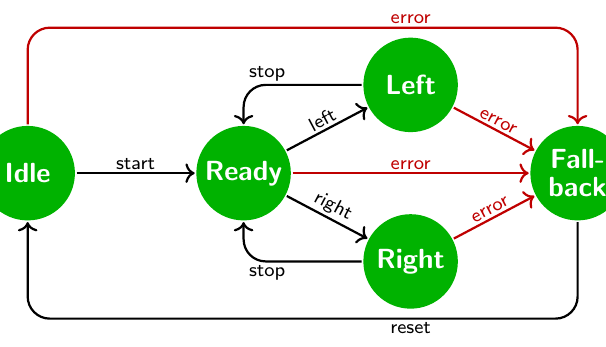
\begin{tikzpicture}
    \tikzstyle{nd}=[circle,white,fill=green!70!black,
      align=center,very thick, minimum width=12mm,inner sep=1pt,
      font=\bfseries\sffamily]
    \node[nd](idle){Idle};
    \node[nd,right=1.5 of idle](ready){Ready};
    \coordinate[right=1.5 of ready](move);
    \node[nd,above=0.5 of move](left){Left};
    \node[nd,below=0.5 of move](right){Right};
    \node[nd,right=1.5 of move](error){Fall-\\[-2pt]back};
    %
    \coordinate[xshift=-10pt](start)at(idle.west);
    \coordinate[yshift=3pt](top)at(left.north);
    \coordinate[yshift=-3pt](bot)at(right.south);

    \tikzstyle{arr}=[->,thick,font=\scriptsize\sffamily,sloped,
                     inner sep=1pt,rounded corners=8pt]
    \tikzstyle{err}=[color=red!75!black]
    \draw[arr]
      (idle) edge[<-] (start)
      % (init)edge node[above]{all-ok}(idle)
      (idle)edge node[above,black](start){start}(ready)
      (ready) edge node[above]{left}(left)
              edge node[above]{right}(right)
              edge[err] node[above]{error}(error)
      (left)  edge[err] node[above]{error}(error)
      (right) edge[err] node[above]{error}(error);
    \draw[arr] (error) |- (bot) node[below]{reset} -| (idle);
    \draw[arr,err] (idle) |- (top) node[above]{error} -| (error);
    % \draw[arr] (idle) |- (top)                    -| (error);
    % \draw[arr,red] (st) -| (start) |- (top)      -| (error);
    \draw[arr] (left) -| node[above,pos=0.4]{stop} (ready) ;
    \draw[arr] (right) -| node[below,pos=0.4]{stop} (ready) ;
    % \draw[arr,bend right] (idle) edge (st)
                          % (st) edge (idle);
    % \draw[arr] (idle) edge[white,-,line width=4pt] (ready) edge (ready);

    \pgfresetboundingbox
    \draw [draw=none] (idle|-top) rectangle (error|-bot);
  \end{tikzpicture}
  \caption{General behaviour of the controller component}
  \label{fig:motor-controllor-beh}
\end{figure}

The \compn{controller} then checks every 400ms if the \compn{motor} reached the movement \chn{limit} or if it detected some \chn{error}. This check is made using a shared register between the \compn{motor} and the \compn{controller}.
If the \compn{controller} detects that the limit is reached between 4000ms and 5000ms after the move instruction is sent, it becomes idle and notifies the \compn{dashboard}. Otherwise it 
raises an \chn{error} (more info on this below) and goes to a fallback state.
%
If the motor is misbehaving, it should not take more than 6000ms to raise an error since the move-instruction is sent.
While in a fallback state, the \compn{controller} waits for the \compn{dashboard} to send a \chn{reset} command to become idle again.


\myparagraph{Raising errors}
Everytime an error is raised by the \compn{controller}
an \chn{error} message must be sent to the dashboard and
a \chn{stop} message must be sent to the \compn{motor}.

\myparagraph{Three components with global constants}
The \compn{controller}'s core behaviour is described above. The \compn{dashboard} and the \compn{motor} will be also modelled as two dedicated timed automata.
 % but we would like to have multiple implementations: one for each \textbf{scenario} (or a parameterised version of each).
% Model at least a pair of \compn{dashboard} and \compn{motor} that behave well, i.e., interact in an expected way, and a pair that misbehaves and forces the system to reach a fallback state. You can model more scenarios to capture corner cases.
  Your model should be parameterised by (at least) the following global constants:
\begin{itemize}
  % \item Maximum attempts;
  \item Minimum and maximum time at the idle and start phase;
  \item Minimum and maximum time to expect the limit to be reached;
  \item Periodicity to read the status of the the motor;
\end{itemize}




\begin{myExercise} \label{ex:model}
  Model this system as an UPPAAL model and \textbf{submit} it to the repository.
  We would like to have multiple versions: one for each \textbf{scenario}.
  % (or a parameterised version of each).
  Each scenario will include a \compn{controller} and/or a \compn{motor} with different behaviour. 
  Model at least two scenarios:
  \begin{itemize}
    \item when both \compn{dashboard} and \compn{motor} behave well, i.e., never lead the system to a fallback state;
    \item when the motor misbehaves, i.e., leads the system to a fallback state.
  \end{itemize}
  You can model more scenarios to capture different cases when the system behaves well or misbehaves. \textbf{Describe} this UPPAAL model and the 3 scenarios in your report,
\textbf{justifying} clearly your decisions (assumptions and abstractions) made in this modelling exercise.

%   , including at least three scenarios....
%   Include three concrete scenarios of this controller, i.e., assume that the dashboard performs three different fixed sequences of instructions at specific points in time.
%   This is an open task: you should implement at least a \compn{controller}, a \compn{motor}, and a \compn{dashboard}, and you may use extra automata if needed. You can also include new assumptions or functionality, provided that you explain them.

%   Your model should be parameterised by (at least) the following global constants:
% \begin{itemize}
%   % \item Maximum attempts;
%   \item Minimum and maximum time at the idle and start phase;
%   \item Minimum and maximum time to expect the limit to be reached;
%   \item Periodicity to read the status of the the motor;
% \end{itemize}
% \end{myExercise}



% \myparagraph{Critical implementation with 2 controllers}
% \textbf{MOVE: ask to model the one above, and then a simpler 2-controller version check the last state at the ready state. THe dashboard will send the same message to both, but the motor can send different messages (e.g., at different times).}

% A more complex version of this system uses 2 \compn{controllers} for redundancy, both interacting with the \compn{dashboard} and the \compn{motor}.
% Every 100ms each of the two \compn{controllers} should check if the other controller is in the same state, using shared variables. After 3 failed attempts this controller should raise an error and go to its fallback state.

% To be able to test this pair of \compn{controllers}, the \compn{dashboard} can also send a \chn{fail} command to any of the \compn{controllers}, rendering it useless.
% Once a controller is faulty, it should not take more than 6000ms to raise an error since a successful \emph{start}, \emph{left}, or \emph{right} instruction is sent, or a movement \emph{limit} is reached.

\end{myExercise}



% \[\includegraphics[width=\textwidth]{RFID-conveyor.pdf}\]

% \begin{myExercise} \label{ex:req}
%   Write a set of 5 or more desirable requirements following the EARS approach based on the description of this system. If you want, you can make new assumptions not described above, making it explicit what is new.
% \end{myExercise}



% \begin{myExercise} \label{ex:model}
%   Model this system as an UPPAAL model \textbf{without} the extension of the second controller.
%   Include three concrete scenarios of this controller, i.e., assume that the dashboard performs three different fixed sequences of instructions at specific points in time.
%   This is an open task: you should implement at least a \compn{controller}, a \compn{motor}, and a \compn{dashboard}, and you may use extra automata if needed. You can also include new assumptions or functionality, provided that you explain them.

%   Your model should be parameterised by (at least) the following global constants:
% \begin{itemize}
%   % \item Maximum attempts;
%   \item Minimum and maximum time at the idle and start phase;
%   \item Minimum and maximum time to expect the limit to be reached;
%   \item Periodicity to read the status of the the motor;
% \end{itemize}
% % Note that there may be several approaches, some more detailed than others, to model this system. 
% Describe this UPPAAL model and the 3 scenarios in your report,
% justifying clearly your decisions (assumptions and abstractions) made in this modelling exercise.
% \end{myExercise}



\begin{myExercise} \label{ex:model2}
% \myparagraph{Critical implementation with 2 controllers}
% \textbf{MOVE: ask to model the one above, and then a simpler 2-controller version check the last state at the ready state. THe dashboard will send the same message to both, but the motor can send different messages (e.g., at different times).}
For safety reasons, these systems need redundancy to reduce the chances of failure.
A safer system is a variation of the model above that
% A more complex version of this system
uses 2 \compn{controllers} for redundancy, both interacting with the \compn{dashboard} and the \compn{motor}.

While in states \texttt{Ready}, \texttt{Left}, and \texttt{Right} (c.f. \cref{fig:motor-controllor-beh}, the two \compn{controllers} check if they are consistent. More specifically, every 100ms each of the two \compn{controllers} should check if the other controller is in the same state, using shared variables. After 3 failed attempts this controller should raise an error and go to its fallback state.

Furthermore, the \compn{motor} uses two different channels (or shared variables) to send information to the two \compn{controllers} (which may be inconsistent in a faulty scenario).

% To be able to test this pair of \compn{controllers}, the \compn{dashboard} can also send a \chn{fail} command to any of the \compn{controllers}, rendering it useless.
% Once a controller is faulty, it should not take more than 6000ms to raise an error since a successful \emph{start}, \emph{left}, or \emph{right} instruction is sent, or a movement \emph{limit} is reached.

Create an updated model of this system and \textbf{submit} it to the repository.
  % Create an updated model based on the previous one that uses 2 controllers, as explained above.
%
As before, model at least two concrete scenarios, of a successful and an unsuccessful execution.
 % as before, but now also considering fault injections.
\textbf{Describe} this UPPAAL model and the 3 scenarios in your report,
\textbf{justifying} clearly your decisions (assumptions and abstractions) made in this modelling exercise.
%   Your model should be further parameterised by (at least) the following global constants:
% \begin{itemize}
%   \item Number of attempts to incorrectly detect a wrong state before raising an error;
%   \item Periodicity to check for the state.
%   % \item Minimum and maximum time at each phase;
% \end{itemize}
% % Note that there may be several approaches, some more detailed than others, to model this system. 
% Describe this new UPPAAL model and the 3 scenarios in your report,
% justifying clearly your decisions (assumptions and abstractions) made in this modelling exercise.
\end{myExercise}


\begin{myExercise} \label{ex:ctl}
  Use UPPAAL's CTL logic to express and verify properties.
  \subex{ \label{ex:ctl-req}
  % Specify all properties from the requirements in \cref{ex:req}.
  Formulate 4 properties of one of the systems above based on their descriptions. If you want, you can make new assumptions not described above, making it explicit what is new.
  }

  \subex{Express a property in UPPAAL's CTL logic for each item below. Fix a particular set of parameters (c.f. the problem description), and say if each property holds or not for your model (or if it takes too much time), and explain why.
  \begin{enumerate}
    \item It is possible to move the engine 3 time to the left in less than 15000ms;
    \item Whenever a fallback state is reached, it must take at least 6000ms until the motor can turn again to the left.
    \item Until a scenario is finished, the system does not deadlock.
  \end{enumerate}
  }

  % \subex{Select 5 properties from \cref{ex:ctl-req}, and for each of them find different values for the parameters that satisfy and that reject them. Use the model from \cref{ex:model2} if available, or from \cref{ex:model} otherwise. If a given property is always true of false, justify informally why.}

\end{myExercise}




 
\end{document}